\chapter{Bewertung}
\label{sec:bewertung}
In diesem Kapitel wird die Webanwendung anhand eines Fragebogens insgesamt von vier Personen bewertet. Alle vier Personen haben eine Position im Unternehmen inne. Die Information über den Namen vom jeweiligen Bewerter sowie seine Position im Unternehmen wird aus Datenschutzgründen nicht angegeben. Mit Hilfe des Online-Tools AttrakDiff\footnote{\url{http://attrakdiff.de/}} wurde der Fragebogen erstellt.\bigskip

Allgemein betrachtet sind die Ergebnisse aus dem Fragebogen zufriedenstellend ausgefallen. Besonders positiv ausgefallen sind die Ergebnisse in puncto Farbigkeit. Vor allem die eingesetzten Farben wurden von den Bewertern positiv bewertet. In Bezug auf die Vielseitigkeit blieb die Bewertung hinter den Erwartungen zurück. Die Seite wirkt nicht abwechslungsreich genug und auch die Seitengestaltung ist zu eintönig. Ebenfalls in Sachen Geschicklichkeit wurde ein positives Feedback von den Bewerten erwartet. Leider blieben die Ergebnisse hinter den Erwartungen zurück.\bigskip

Aus dem Feedback wurden einige Verbesserungsvorschläge herausgearbeitet . Zum Beispiel soll überlegt werden, wie das Layout zukünftig verbessert werden kann, so dass es bei den Anwendern einen guten Eindruck hinterlässt.

\begin{figure}[H]
  \begin{center}
    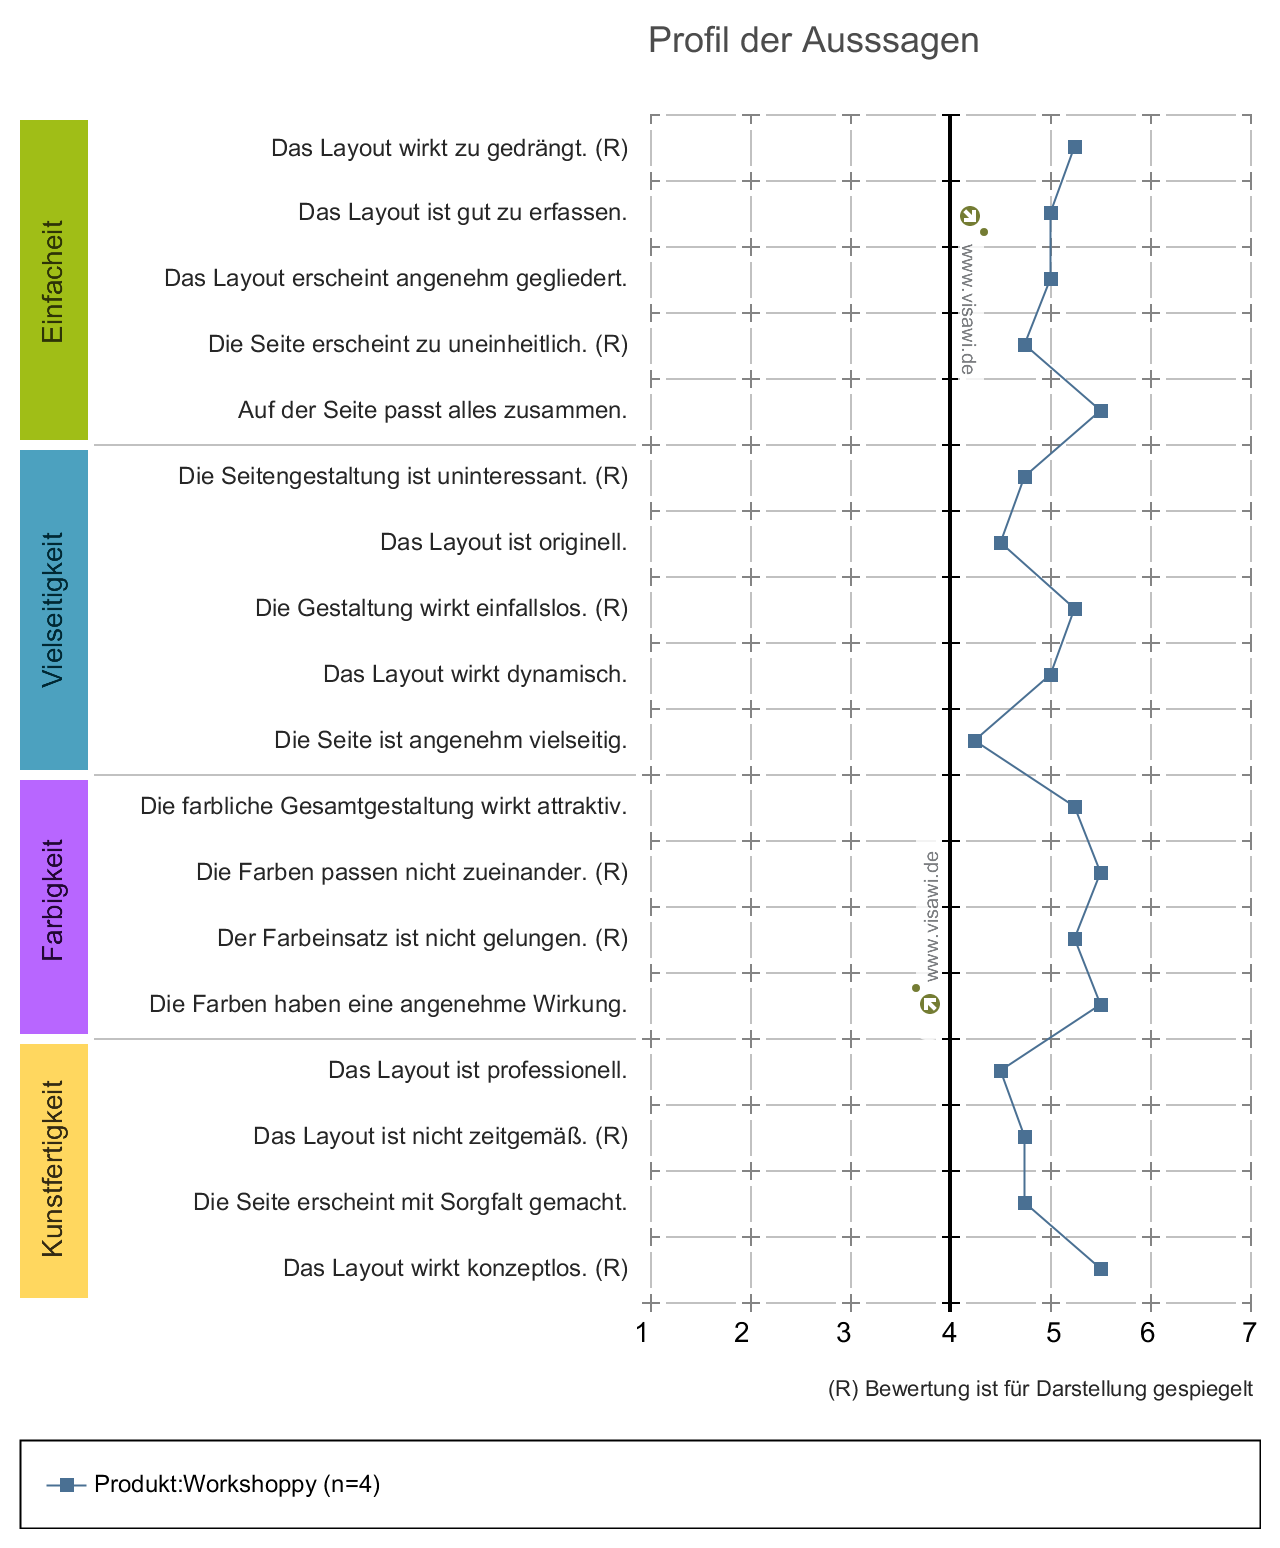
\includegraphics[scale=0.3]{img/das_Profil_der_Aussagen}
	\caption{Ergebnisse aus den Fragebogen} 
	\label{fig:profil der Aussagen}
  \end{center}   
\end{figure}

\begin{figure}[H]
  \begin{center}
    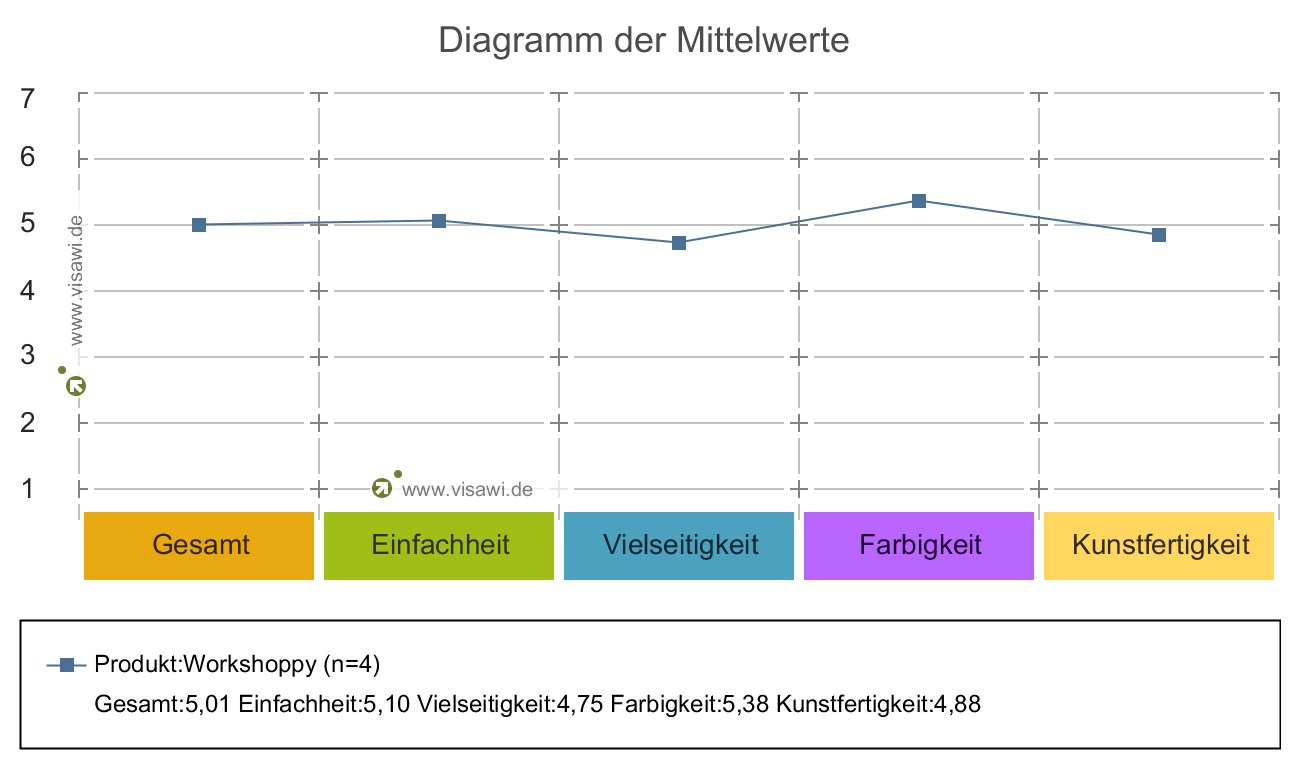
\includegraphics[scale=0.3]{img/Diagramm_der_Mittelwerte}
	\caption{Ergebnisse aus den Fragebogen} 
	\label{fig:Diagramm_der_Mittelwerte}
  \end{center}   
\end{figure}